\documentclass[tocnosub,noragright,centerchapter,12pt,fullpage]{uiucecethesis09}


% Use draftthesis for notes and date markings on every page.  Useful when you
%   have multiple copies floating around.
% Use offcenter for the extra .5 inch on the left side. Needed with fullpage and fancy.
% Use mixcasechap for compatibility with hyperref package, which does NOT like all caps default
% Use edeposit for the adviser/committee on the title page.
% Use tocnosub to suppress subsection and lower entries in the TOC.
% PhD candidates use "proquest" for the proquest abstract.

\makeatletter

%%%%%%%%%%%%%%%
% MK Added to make bib work
% \bstctlcite{IEEEexample:BSTcontrol}

% MK added to highlight stuff
\usepackage{color,soul}

% MK added so figures can use the [H] option and be put where I want them.
\usepackage{float}

% MK added so algorithms work
\usepackage{algorithm}

%%%%%%%%%%%%%%%

\setcounter{secnumdepth}{5} % to make subsubsections work
\usepackage{setspace}
\usepackage{epsfig}  % for figures
\usepackage{graphicx}  % another package that works for figures
\usepackage{subfigure}  % for subfigures
\usepackage{amsmath}  % for math spacing
\usepackage{amssymb}  % for math spacing
%\usepackage{url}  % Hyphenation of URLs.
\usepackage{lscape}  % Useful for wide tables or figures.
\usepackage[justification=raggedright]{caption}	% makes captions ragged right - thanks to Bryce Lobdell

\DeclareMathOperator*{\argminA}{arg\,min} % Jan Hlavacek

% Uncomment the appropriate one of the following four lines:
%\phdthesis
%\phdthesis
%\otherdoctorate[abbrev]{Title of Degree}
%\othermasters[abbrev]{Title of Degree}

\title{Automated Isotope Identification Using Artificial Neural Networks}
\author{Mark Kamuda}
\department{Nuclear Plasma and Radiological Engineering}
%\department{\mbox{Nuclear, Plasma, and Radiological Engineering}}
\degreeyear{2018}

% Advisor name is required for
% - doctoral students for the ProQuest abstract
% - master's students who do not have a master's committee
% \advisor{Assistant Professor Clair J. Sullivan}

% Uncomment the \committee command for
% - all doctoral students
% - master's students who have a master's committee
\committee{Professor Kathryn Huff, Adviser\\
        Professor Rizwan Uddin\\
        Professor Tomasz Kozlowski\\
        Professor Clair Sullivan\\
        Professor Mark Hasagawa$-$Johnson}





\begin{document}

%%%%%%%%%%%%%%%%%%%%%%%%%%%%%%%%%%%%%%%%%%%%%%%%%%%%%%%%%%%%%%%%%%%%%%%%%%%%%%%
% COPYRIGHT
%
%\copyrightpage
%\blankpage

%%%%%%%%%%%%%%%%%%%%%%%%%%%%%%%%%%%%%%%%%%%%%%%%%%%%%%%%%%%%%%%%%%%%%%%%%%%%%%%
% TITLE
%
\maketitle

%\raggedright
\parindent 1em%

\frontmatter


\begin{abstract}
Abstract goes here.
\end{abstract}

\tableofcontents

\listoftables

\listoffigures

\mainmatter


\chapter{Introduction}

The main question addressed in this work is: Can artificial neural networks (ANNs) using simulated spectra as training data automate isotope identification and quantification? Gamma$-$ray spectroscopists often use intuition when identifying isotopes in spectra. ANNs mimic this abstract analysis, synthesizing features of a gamma$-$ray spectrum in non$-$intuitive ways. Exploiting this intuition may overcome common hurdles encountered by other isotope identification algorithms. 

% This may give ANNs the ability to identify and quantify isotopes using large isotope libraries practical for domestic nuclear security, operate using low-resolution NaI radiation detectors without knowing the detector calibration or background spectrum.

% The idea to use ANNs first came as a method to exploit a potential data source in post-detonation nuclear forensics. After the device explodes, first responders will likely flood the affected area. Some of these responders will be fitted with gamma-ray spectrometers, the cheapest and most common being some size of NaI(Tl) scintillation crystals. While these crystals produce a gamma-ray spectrum with somewhat poor resolution, their potential ubiquity over heavier, more expensive systems that may require a day to cool (HPGe need liquid nitrogen temperatures to operate. This requires mechanical cooling or a dewar of liquid nitrogen. Regardless of the cooling method, they require about a day to cool if not already at operational temperature.) make them a potential source of a mountain of spectroscopic data from blast debris. This spectroscopic data can be used to identify the isotopes and their ratios in the debris. This data can be used to begin the process of attribution. Currently, the isotopics are calculated by sending debris samples to a few labs around the country (one of which is the Counting Room in the C-NR division at LANL). The debris is then chemically separated into constituent fission products, and those fission products are counted using well shielded HPGe detectors to very accurately determine isotopics. While this process will result in a more accurate measure of debris isotopics, the time necessary to transport, perform the chemical separation for each piece of debris, and measure the debris with the HPGe detectors may be on the order of days. While this may sound quick, this time will sacrifice some of the short-lived isotopes in the debris. In addition to this, if attribution time can be shortened from days to hours, international response could be organized quicker. 

% Current gamma-ray spectroscopy techniques may be inadequate to be used for post-detonation debris analysis. Feature extraction techniques typically rely on fitting non-overlapping gamma-ray peaks. In post-detonation debris, many isotopes will be emitting gamma-rays, creating multiple overlapping gamma-lines. Template matching algorithms may need an excessively large library to handle this task. Each sample of debris will contain tens of isotopes in complicated combinations. These exact combinations may be hard to determine  \textit{a priori} due to differences in device design and fractionation effects. 



The proposed work will demonstrate the performance of ANNs for automated gamma$-$ray spectroscopy in low$-$resolution spectra. The low$-$resolution detector of interest in this work is a 2$-$inch by 2$-$inch NaI(Tl) cylindrical scintillation detector. This detector is industry standard due to its ease of use, low cost, and acceptable resolution for gamma$-$ray spectroscopy. 

The algorithms performance will be displayed on three different datasets. The first dataset will focus on identifying isotopes in ANSI N42$-$34$-$2006, the american national
standard performance criteria for hand$-$held instruments for the detection and identification of radionuclides \cite{ANSI}. The second dataset will focus on 

This ANSI standard also requires isotope identification algorithms to operate when the radioactive material is behind shielding.

% This may give ANNs the ability to identify and quantify isotopes using large isotope libraries practical for domestic nuclear security, operate using low-resolution NaI radiation detectors without knowing the detector calibration or background spectrum.

% Tasks investigated here will focus on identifying isotopes in the ANSI N42-34-2006 required list \cite{ANSI}. This ANSI standard also requires isotope identification algorithms to operate when the radioactive material is behind shielding. Accordingly, the impact of shielding will also be incorporated into this work. 

In addition to isotope identification, this work will explore the ability of ANNs to quantify the count contribution from each isotope. The ANN's ability to extract count contribution information from gamma$-$ray spectra is important for nondestructive analysis (NDA). While NDA is useful for. The second purpose is a possible use of neural networks in post$-$detonation nuclear forensics. In post$-$detonation nuclear forensics, a large number of radioactive fission products are created. Quantifying the amount of isotopes in post$-$detonation debris can yield useful information about the device's properties. Mixtures of laboratory sources will be used as a surrogate for post$-$detonation debris and the ability for the ANN to accurately calculate the mixture components will be established.   

Another case where knowing the isotope quantities in a mixture of isotopes is in uranium enrichment calculations. Knowing the enrichment of uranium is important in two areas. The first are is when uranium is identified at a border crossing. Typically the spectrum would need to be given to a trained spectroscopist to quantify the enrichment, but this process could be automated on the device first used to identify it. The second case would be in treaty verification technologies. Low$-$resolution NaI gamma$-$ray detectors decrease the amount of possibly sensitive information while giving enough information to produce accurate enrichment quantification. The fact that ANNs can be taught to ignore certain patterns and only give information agreed upon by treaty signatories also makes them a good tool for treaty verification. The ability of ANNs to operate without knowing the shielding and background spectrum makes them better for zero knowledge scenarios. NaI detectors also have a higher efficiency than the higher resolution HPGe. This means that the counting times for NaI are smaller than would be required to get the same number of counts using an HPGe. 





% An ANN will learn to perform these tasks by learning from simulated datasets that represent these tasks. The aim of this work is to demonstrate that an ANN can be taught to perform different isotope identification tasks using a simulated dataset using the same general training method.









\chapter{Literature Review}


\section{Gamma$-$Ray Spectroscopy for Isotope Identification}

Traditionally, isotope identification is conducted by a trained spectroscopist. Rawool$-$Sullivan et al. identified a common workflow performed by a group of gamma$-$ray spectroscopists \cite{Sullivan2010}. This workflow included discriminating background and source photopeaks, adjusting the calibration using background photopeaks and checking for shielding effects in the low$-$energy photopeaks. Once photopeaks are identified, the spectroscopist would use their prior knowledge of isotope emissions (or consult a database of these emissions) to match isotopes to the spectrum. The researchers also noted that while  spectroscopists used this book knowledge, they often would use intuition developed from analyzing tens or hundreds of gamma$-$ray spectrum. The researchers also noted the difficulty in incorporating this subjective analysis into an automated algorithm.
% This is one of the main arguments for using ANNs in automated isotope ID


There are many automated radioisotope identification methods available, but few perform well given a low$-$resolution gamma$-$ray spectrum of a mixture of radioisotopes. Common methods include library comparison algorithms, region of interest (ROI) algorithms, principle component analysis (PCA), and template matching.

Library comparison algorithms attempt to match photopeak energies found in a gamma$-$ray spectrum with those found in a library of known isotope decay energies. Drifts and uncertainties in detector calibration can lead to misidentifying photopeaks, leading to incorrect isotope identifications \cite{burr2009}. To be automated, this method needs an algorithm to extract photopeak centroids from a spectrum. Photopeak extraction algorithms face difficulties when a large number of photopeaks overlap in a spectrum, such as when a mixture of radio$-$isotopes are measured with a low$-$resolution detector \cite{xiong2015}.

ROI algorithms search for elevated counts compared to background in a region where photopeaks are expected to be for different radioisotopes. ROI algorithms may also operate poorly when photopeaks of different radioisotopes overlap \cite{burr2009}. For this reason, large isotope libraries will preform poorly using this method. Similarly to the library comparison algorithm, calibration drift may shift photopeaks into different neighboring ROIs, leading to incorrect identification. The ROI method has been used to differentiate normally occurring radioactive material (NORM) from special nuclear material (SNM) using plastic scintillators \cite{Ely2006}.

PCA can also be applied to radioisotope identification. The goal of PCA is to reduce the dimensionality of a dataset into uncorrelated variables \cite{Jolliffe2002}. Using a few of these principle components, the data may be represented in a reduced space that contains most of the information present in the original data. The transformed data can then be clustered based on isotope identity. Clustering algorithms may include K$-$means or Mahalanobis distance \cite{Kanungo2002, Kumari2012}. PCA has been applied to isotope identification using plastic scintillators \cite{Boardman2012} and anomaly detection using both plastic scintillators and NaI detectors \cite{runkle2006b}. Despite the progress of PCA in some isotope identification problems, there has not been significant progress in applying PCA to separating mixtures of isotopes in gamma$-$ray spectra.

Template matching algorithms find an example in a database of gamma$-$ray spectra that most closely matches a measured spectrum \cite{burr2009}. The database of spectra can contain multiple detector calibration settings, shielding materials, and source$-$to$-$detector distances. Goodness of fit can be measured using a hypothesis test such as chi$-$squared test, euclidean distance, or Mahalanobis distance. While a sufficient amount of example spectra can be used to identify almost any measured spectrum, the drawback of this method is the time necessary to compare a measured spectrum to the library and the computer memory necessary to store said library. This method also may have difficulty when mixtures of isotopes are considered, although work is being done to correct this \cite{mattingly2010}.

These algorithms largely incorporate book knowledge. By further incorporating the intuition identified by Rawool$-$Sullivan et al., these algorithms may be improved. A machine learning approach to automated gamma$-$ray spectroscopy may be able to marry book knowledge and a trained spectroscopists intuition.  




\section{Artificial Neural Networks}

Artificial neural networks were first created to mimic biologic neurons. Since their creation, they have demonstrated promising results on a variety of different classification and regression tasks \cite{Jeyanthia2015, Krizhevsky2012, Rababaah2015}. The following sections will give an overview of how ANNs learn and operate.


\subsection{Architecture and Training}

ANNs work by mapping arbitrary input spaces, $\mathbb{R}^N$, to arbitrary output space, $\mathbb{R}^K$. An example one hidden layer ANN mapping $\mathbb{R}^N$ $\mapsto$ $\mathbb{R}^K$ is shown in Figure \ref{fig:Network}. Each circle represents a neuron, or node. The mathematical process governing each neuron in the ANN is shown in Figure \ref{fig:Node}. In Figure \ref{fig:Node}, the signal from the previous layer is propagated to the next by applying some function, typically sigmoidal, to the dot product of the signal from the previous layer and the weight vector going into a given node, B$_{j}$ in Figure \ref{fig:Node}. Given a one$-$layer ANN with a finite number of hidden nodes, any function $\mathbb{R}^N$ $\mapsto$ $\mathbb{R}^K$ can be described to arbitrary precision \cite{hornik1991}. Additional hidden layers increase the representational power of an ANN, reducing the number of nodes and computational power required to represent a function. There is no direct method to compute the optimal number of hidden layers or nodes for a given problem. These, along with other hyperparameters, need to be optimized for a given dataset.

\begin{figure}
    \centering
    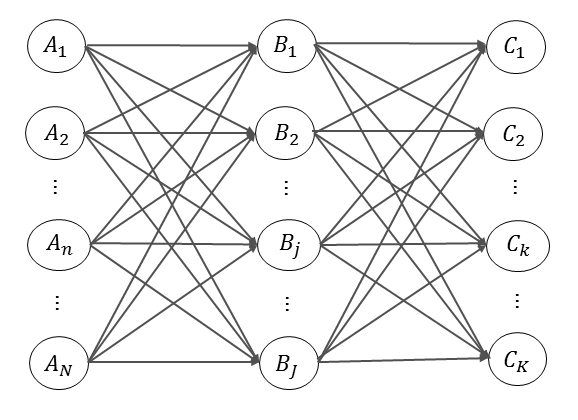
\includegraphics[width=0.5\linewidth]{images/Network}
    \caption{Example ANN with input layer A, hidden layer B, and output layer C.}
    \label{fig:Network}
\end{figure}

\begin{figure}
	\centering
	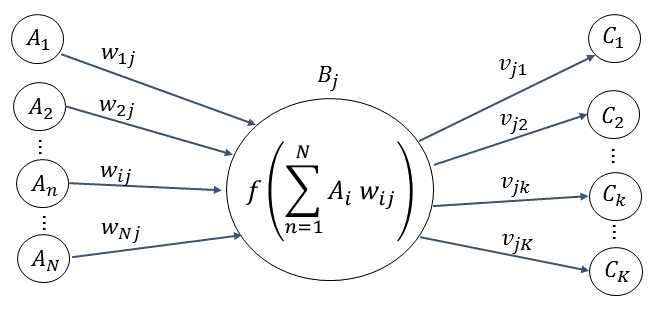
\includegraphics[width=0.65\linewidth]{images/Node_ABC_2}
	\caption{Summary of the operation of a single neuron.}
	\label{fig:Node}
\end{figure}

Artificial ANNs learn a function by changing the weights connecting the layers so that some error function is minimized for a given dataset. One popular method to update the weights is through the process of gradient descent through the backpropogation of errors \cite{Rumelhart1986}. The update equation for a single weight, $w_j$, is shown in Equations \ref{eq:update1} and \ref{eq:update2}. In these equations, $E$ is the given error function to be minimized (commonly mean squared error or cross entropy) and $\eta$ is the learning rate of the ANN.


\begin{equation} \label{eq:update1}
\Delta w_{j} = - \eta \frac{dE}{dw_j}
\end{equation}

\begin{equation} \label{eq:update2}
w^{new}_{j} = w^{old}_{j} + \Delta w_{j}
\end{equation}

\subsection{Hyperparameters}

In general, ANNs have a tendency to memorize their training set in a process called overtraining. An overtrained ANN will tend to incorrectly identify novel data. To prevent this, a number of hyperparameters were used to prevent overfitting and optimize performance. Unfortunately, there is currently no known method to know which hyperparameters have an impact on model performance before training. Because of this, a number of popular hyperparameters are typically added to a model and a random hyperparameter search is used to identify those which are important. \iffalse Because there is no direct method to identify which hyperparameters are important or what their values should be, a random hyperparameter search can be used to find a close$-$to$-$optimal network structure and hyperparameter values.\fi There is evidence that a random search in a given hyperparameter range finds better hyperparameters quicker than a grid search in the same range \cite{Bergstra2012}. There is also a proof showing that given 60 points randomly sampled in some space with a finite minimum, the minimum of those 60 random samples is within 5\% of the true minimum with 95\% probability \cite{Zheng2015}. Training 60 ANNs is computationally feasible, making this a good method to find a close$-$to$-$optimal ANN for a given dataset. 



\section{Automated Isotope Identification Using ANNs}

There have been a number of published papers which apply ANNs to automated isotope identification. ANNs have been applied to peak fitting \cite{Abdel-Aal2002}, isotope identification \cite{Abdel-Aal1996, Medhat2012}, and activity estimation \cite{Abdel-Aal1996, Vigneron1996}. Many of this work rely on ROI methods \cite{Pilato1999}, feature extraction \cite{Chen2009}, high$-$resolution gamma$-$ray spectra as the input to the ANN \cite{Yoshida2002}, small libraries of isotopes, and assume perfectly calibrated detectors. ANN training methods created for high$-$resolution gamma$-$ray spectra may not perform well when trained using low$-$resolution spectra given the large discrepancy in resolution. ANN training that relies on ROI methods may not perform well when ROIs overlap significantly with large libraries of isotopes.

It has been shown that an ANN may be trained to perform isotope identification and quantification using low$-$resolution NaI gamma$-$ray spectrum using a library of five isotopes \cite{Olmos1991}. While promising, this study did not include complicated source mixture analysis. This study also used a library too small to be of practical use. The American National Standards Institutes (ANSI) has identified 31 gamma$-$ray emitting isotopes that automated isotope identification algorithms should be able to identify \cite{ANSI}.


\chapter{Artificial Neural Network Approach to Identifying and Quantifying isotopes in Gamma$-$Ray Spectra}


\section{Introduction}

The ANN presented here is trained to quantify the count contribution of each isotope from a library. Because the ANN trains using simulated gamma$-$ray spectra, additional datasets can be trivially created. The ANN structure, training details, and hyperparameter optimization are described. 


\section{Artificial Neural Network Structure}

The fully connected ANN explored in this work uses a rectified linear ($relu$) activation function, seen in Equation \ref{eq:relu}, with a $softmax$ output function, seen in Equation \ref{eq:softmax}.

\begin{equation} \label{eq:relu}
relu(x) = max(0,x).
\end{equation}

\begin{equation} \label{eq:softmax}
softmax(z_j ; \boldsymbol{z}) = \frac{\exp(z_j)} {\sum_{k=1}^{K} \exp(z_k)}.
\end{equation} 

The $relu$ function was chosen for the node activations because previous work has shown that it is easy to optimize and generally perform better than other non$-$linear functions \cite[pg. 189]{Goodfellow-et-al-2016}. While the $softmax$ function is traditionally used in classification ANNs, using it here ensures the output from the ANN is normalized to unity. This allows the ANN to output relative count contributions from each isotope. This method was shown to perform well for quantifying isotopes in real and simulated spectra \cite{kamudaThesis2017,kamuda2017}. By setting a detection threshold based on the highest count contribution, this method can also be used as an identification algorithm. For example, Table \ref{table:top_five} shows the top five isotope outputs from an ANN that used the spectrum in Figure \ref{fig:top_five} as input. Using an arbitrary threshold of 15\%, any isotope with a contribution below 15\% of 0.441 can be ignored. This leads to a correct identification of $^{60}$Co, $^{137}$Cs, and background. The threshold used can be chosen to ensure a desired performance metric (false alarm rate, precision, recall) on an appropriate dataset. 

\begin{table}[H]
\centering
\caption{Top five isotopes found by an ANN trained to quantify isotopes. }
\label{table:top_five}
\begin{tabular}{|c|c|}
\hline
Isotope    & \begin{tabular}[c]{@{}c@{}}Count \\ Contribution\end{tabular} \\ \hline
$^{60}$Co  & 0.441                                                         \\ \hline
$^{137}$Cs & 0.440                                                         \\ \hline
Background & 0.068                                                         \\ \hline
$^{99}$Mo  & 0.019                                                         \\ \hline
$^{235}$U  & 0.017                                                         \\ \hline
\end{tabular}
\end{table}

\begin{figure}[H]
    \centering
    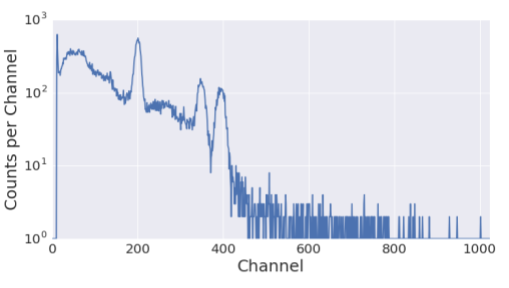
\includegraphics[width=0.7\linewidth]{images/CoCs_mix}
    \caption{Gamma$-$ray spectrum of a 0.288 $\mu$Ci $^{60}$Co source and a 0.890 $\mu$Ci $^{137}$Cs source. Each source$-$to$-$detector distance was adjusted so their respective count rate on the detector was equal.}
    \label{fig:top_five}
\end{figure}


\section{Dataset Construction}

In order to train an ANN, a training set and training key must be provided. The training set is a set of ANN input data and the training key is the correct ANN output for each input. Because creating a training set of real gamma$-$ray spectra is infeasible, the training set used in this work was simulated. The training set was created using a one$-$dimensional Monte Carlo radiation detector simulation program called GADRAS \cite{mitchell2014}. The simulation process began by simulating individual 1 mCi sources with no background. Each source was simulated at a distance of 30cm from a 2 inch by 2 inch Ortec 905$-$3 NaI spectrometer for 10 hours, ensuring each spectrum had low statistical noise. These single isotope sources were then sampled using the inverse transform sampling method \cite{Devroyne}. This allows the creation of arbitrary source combinations. The background isotopes were modeled using built$-$in GADRAS background sources for $^{40}$K, uranium and daughters in soil, and thorium and daughters in soil.

Because the calibration on NaI detectors shifts over time (due to voltage drift in the electronics and changes in crystal temperature), a method to change training spectra calibration was included. To mimic gain shift, the channels in each spectrum were linearly rebinned by some percent. The magnitude of each shift was uniformly chosen between a +/- 25\% gain drift. After rebinning, the resulting spectrum was reconstructed using third order spline interpolation with the new bin positions.


Using this method, many training sets can be created depending on different algorithm goals. The training set and isotope library can be modified for specific problems like unknown source interdiction, uranium enrichment calculations, and post$-$detonation nuclear forensic debris analysis. Methods of creating ANNs for these problems will be described in later sections.

% The isotope library chosen for this demonstration was 29 gamma-ray producing isotopes from the ANSI N42.34-2006 standard, as well as $^{152}$Eu \cite{ANSI}. Based on lab observations using an Ortec 905-3 NaI spectrometer, the average background count rate was set at 85 counts per second (cps). Each spectrum in the training set had a maximum of 5 different non-background isotopes included in the spectrum. Each isotope had a count rate which was logarithmically distributed between 10 and 1000 cps. The exposure time was logarithmically distributed between 10 and 2000 seconds. Each isotope, excluding those in background, had an equal probability of being included in each spectrum. The counts from background were distributed uniformly between background thorium, background uranium, and background $^{40}$K.



\section{Training Details and Hyperparameter Optimization}

Once the ANN hyperparameters are decided on, an optimization algorithm is needed to train the model. The Adam optimizer was chosen as the training algorithm for this work due to its incorporation of parts of other successful optimization algorithms and its reported superior performance over these algorithms \cite{Kingma2015}. Another benefit of the Adam optimizer is the introduction of only one additional hyperparameter, the learning rate. Other optimizers require tuning more than one additional hyperparameter. During training, the ANN minimized the average cross entropy,

\begin{equation} \label{eq:CrossEntropy}
E = -{\frac{1} N} \sum_{n=1}^N y_n \log(\hat{y}_n) +  (1-y_n) \log(1-\hat{y}_n),
\end{equation}

between the correct labels, $y_n$, and the network predictions, $\hat{y}_n$. This cost function was chosen because it is traditionally used with ANNs whose output is the $softmax$ function. 


Raw data is typically preprocessed before being input to an ANN. For this work each spectrum was preprocessed by scaling the counts in each bin between [0,1]. Scaling the inputs improves numerical stability during training. 

As previously discussed, hyperparameters are often necessary to properly train an ANN. The following hyperparameters are considered in this study are: the number of neurons in each layer, the number of layers used, initial learning rate for the training algorithm, the $L_2$ weight regularization strength, and neuron dropout rate. 

Adding $L_2$ weight regularization allows the magnitude of the weights to increase only when there is a comparable reduction in the unmodified error function.
%
\begin{equation} \label{eq:L2_Reg}
\tilde{E} = E + \sum_i \lambda w_i^2.
\end{equation}
%
In Equation \ref{eq:L2_Reg}, $w_i$ is the weight between each neuron in the ANN and $\lambda$ is the regularization strength hyperparameter. A larger $\lambda$ will force the ANN to prefer smaller weights connecting the neurons. If $\lambda$ is too small, the model is more likely to overfit. If $\lambda$ is too large, the ANN will preferentially minimize the $L_n$ error, failing to learn the desired task.

Another method to reduce model capacity is neuron dropout. Neuron dropout is the process of temporarily removing a neuron from the ANN architecture during training \cite{Srivastava2014}. The probability that a neuron is removed is called the neuron dropout rate, which is a hyperparameter. By applying dropout throughout training, the ANN's architecture changes every iteration. The makes neuron dropout a cost efficient way to average many different ANN architectures, improving performance.

% To reduce free parameters that might lead to overfitting, the number of neurons in each layer is typically smaller than the size of the input layer, in this case 1024. Another method of   Because  kept below 10$^{4}$.   


\section{Key Results}

Two key results are described in the following section. The first result demonstrates the ANNs ability to correctly identify isotopes in the ANSI library with an unknown calibration.  The second result demonstrates the ANNs ability to identify if an isotope that is shielded by lead.  


To demonstrate gain invariance, 


\begin{figure}[H]
\centering
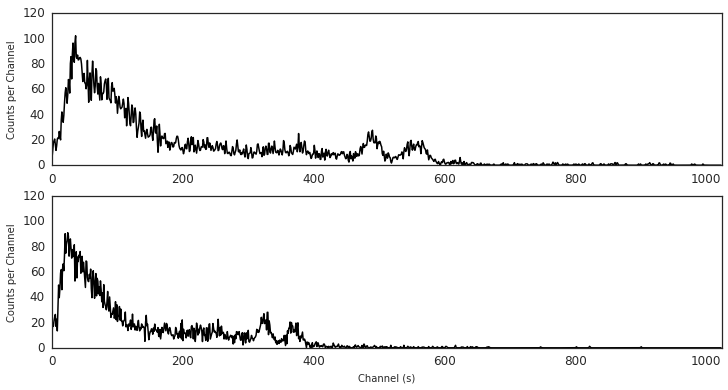
\includegraphics[width=0.75\linewidth]{images/Co60_both_60s}
\caption{Two simulated $^{60}$Co spectra. In each spectrum, the $^{60}$Co and background contribute 5100 counts to the spectrum. The bottom spectrum's gain was offset by -20\% while the top spectrum's gain was offset by +20\%.}
\label{fig:co60_diff_pmt_60s}
\end{figure}




\begin{figure}[H]
\centering
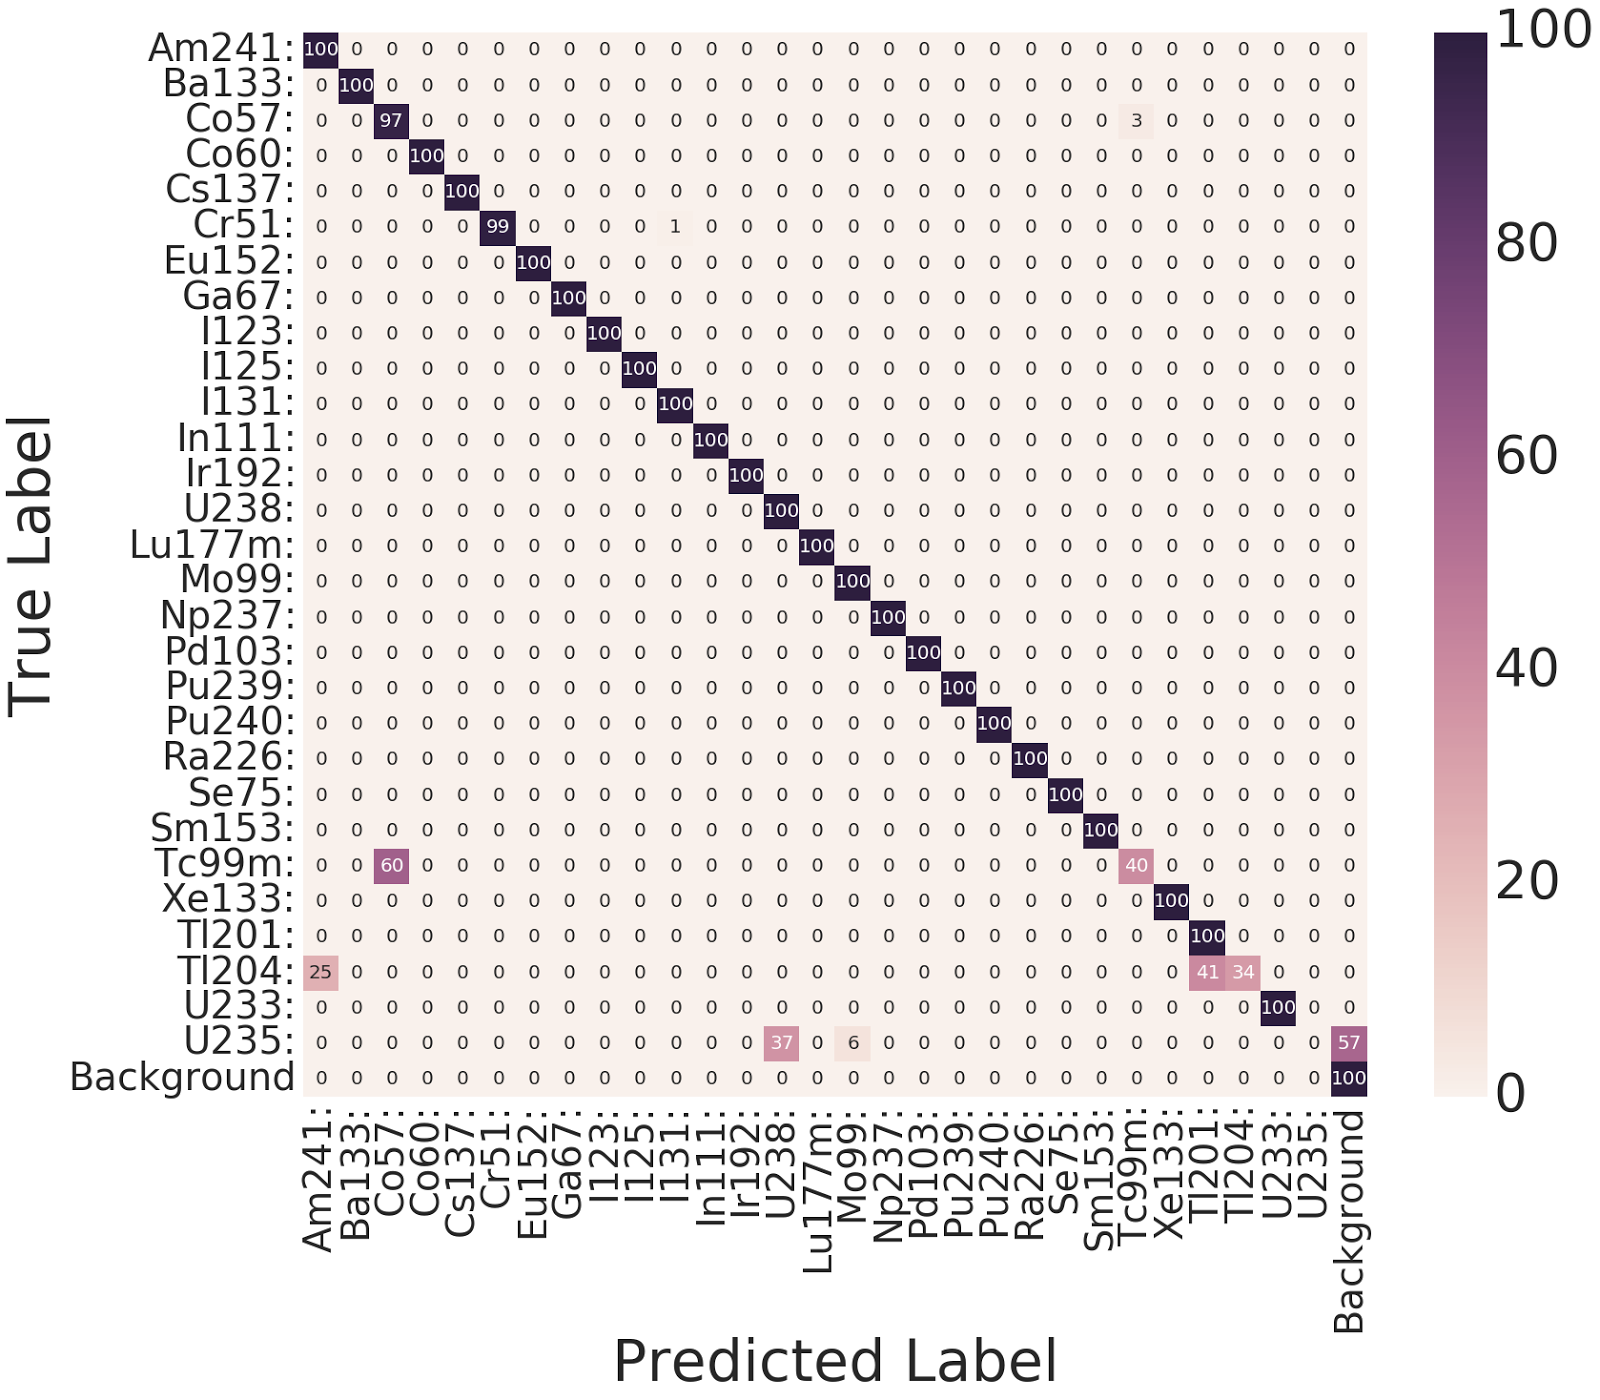
\includegraphics[width=0.7\linewidth]{images/conf_matrix_60s}
\caption{The confusion matrix for a single isotope dataset. Both the source and background contribute 5100 counts to the spectrum.}
\label{fig:conf_matrix_60s}
\end{figure}



\begin{figure}[H]
\centering
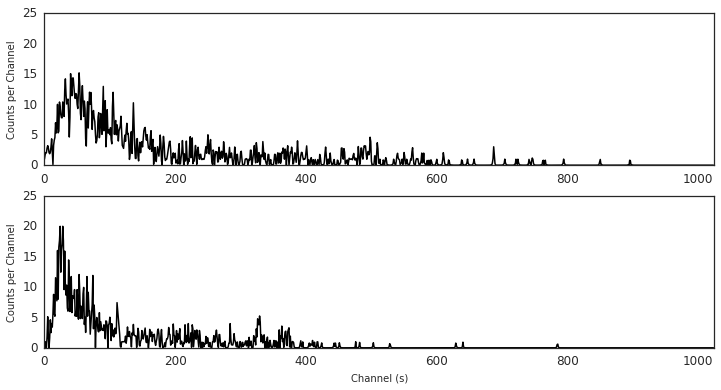
\includegraphics[width=0.75\linewidth]{images/Co60_both_10s}
\caption{Two simulated $^{60}$Co spectra. In each spectrum, the $^{60}$Co source contributes 425 counts and background contribute 850 counts. The red spectrum's gain is offset by -20\%, while the blue spectrum's gain is offset by +20\%.}
\label{fig:co60_diff_pmt_10s}
\end{figure}



\begin{figure}[H]
\centering
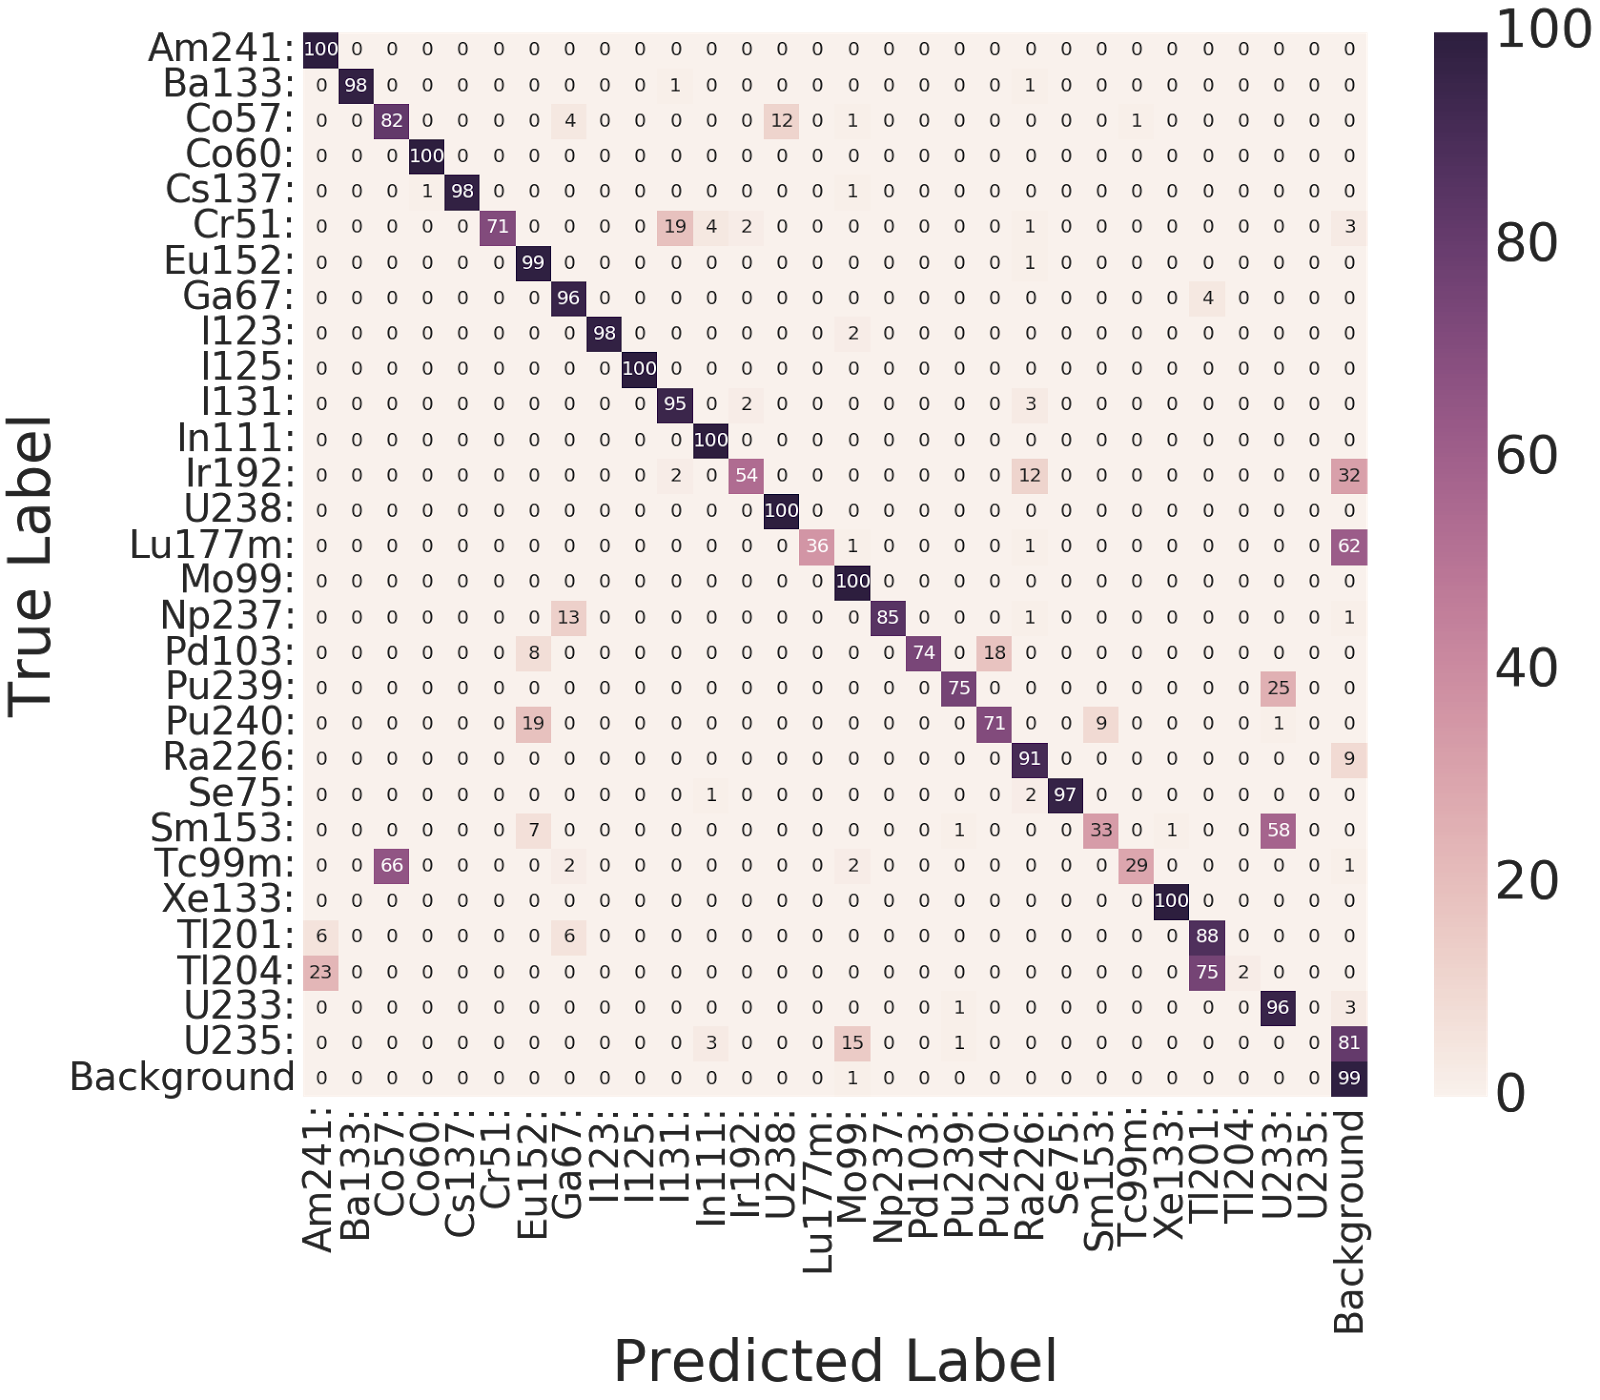
\includegraphics[width=0.7\linewidth]{images/conf_matrix_10s}
\caption{The confusion matrix for a single isotope dataset. In each case, the source contributes 425 counts and background contributes 850 counts to the spectrum.}
\label{fig:conf_matrix_10s}
\end{figure}


An ANN was trained to identify bare and shielded isotopes. The ANN used a training library composed of bare and shielded sources from the ANSI library. 

\begin{figure}[H]
\centering
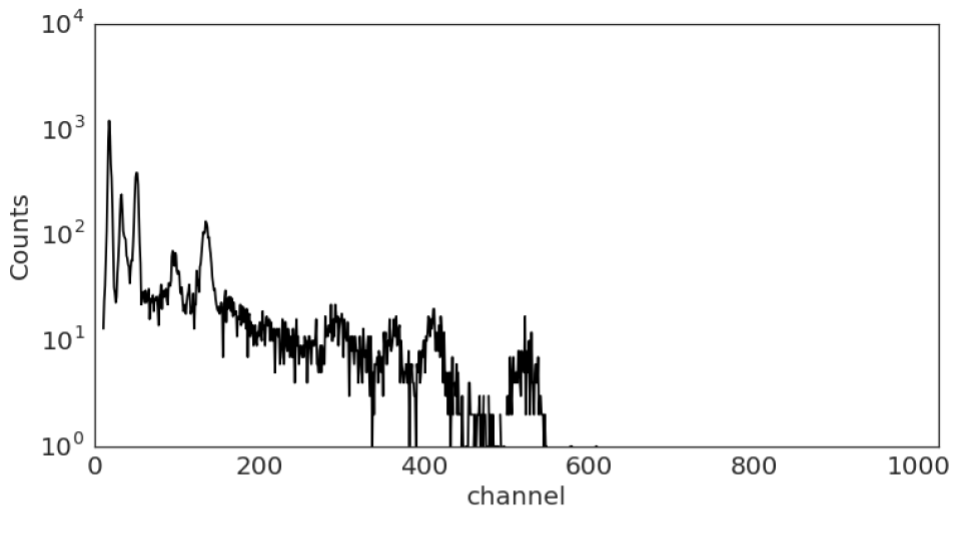
\includegraphics[width=0.75\linewidth]{images/Bare_Eu152}
\caption{Spectra of a Eu152 10μCi source. The collection time for this was 10s.}
\label{fig:Bare_Eu152}
\end{figure}


\begin{table}[H]
\centering
\caption{Average ANN output from five spectra. Each spectrum was collected like the one in Figure \ref{fig:Bare_Eu152}. Only the top five isotopes are shown.}
\label{table:Bare_Eu152_results}
\begin{tabular}{|c|c|}
\hline
Isotope    & \begin{tabular}[c]{@{}c@{}}Count \\ Contribution\end{tabular} \\ \hline
$^{152}$Eu  & 0.496                                                         \\ \hline
Background $^{40}$K & 0.090                                                         \\ \hline
Background Uranium & 0.072                                                         \\ \hline
Background Thorium  & 0.056                                                         \\ \hline
$^{60}$Co  & 0.051                                                         \\ \hline
\end{tabular}
\end{table}



\begin{figure}[H]
\centering
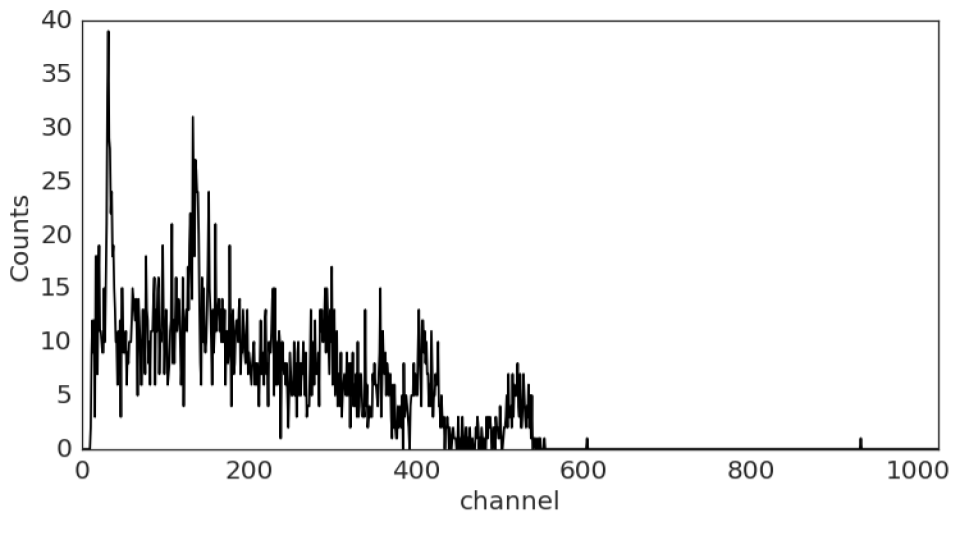
\includegraphics[width=0.75\linewidth]{images/Shielded_Eu152}
    \caption{Spectra of a Eu152 10μCi source. The collection time for this was 10s. The source was shielded by 8mm of lead.}
\label{fig:Shielded_Eu152}
\end{figure}

\begin{table}[H]
\centering
\caption{Average ANN output from five spectra. Each spectrum was collected like the one in Figure \ref{fig:Shielded_Eu152}. Only the top five isotopes are shown.}
\label{table:Shielded_Eu152_results}
\begin{tabular}{|c|c|}
\hline
Isotope    & \begin{tabular}[c]{@{}c@{}}Count \\ Contribution\end{tabular} \\ \hline
Shielded $^{152}$Eu  & 0.303                                                         \\ \hline
Shielded $^{238}$U & 0.234                                                         \\ \hline
$^{137}$Cs & 0.182                                                         \\ \hline
$^{131}$I  & 0.084                                                         \\ \hline
$^{60}$Co  & 0.074                                                         \\ \hline
\end{tabular}
\end{table}








%%%%%%%%%%%%%%%%%%%%%%%%%%%%%%%%%%%%%%%%%%%%%%%%%%%%%%%%%%%%%%%%%%%%%%%%%%%%%%%%%%%%%%%%%%%

% \section{Thesis and TNS Publication}

% The work I published has a lot of room for improvement. Some physics in the MCNP 6 model were neglected, like any radiation contribution from bremsstrahlung and environmental scatter. Also the background isotope spectra were very wrong. These were generated assuming a point source of radiation. Real background is distributed in the soil. Many scattering events in soil along with skyshine contribute to a spectrum that looks very different from a point source. %(cite MCNP background simulation paper). 

% There were parts of the published work that were good. The sampling method based on isotope templates is a good method to simulate lots of realistic gamma-ray spectra. One of the most difficult parts of ANN training is creating a good training set that represents reality. This method can be used to simulate most things, which is hugely useful. The results of the published work were also very promising. Despite the unrealistic physics model used in the simulation, the ANN correctly identified isotopes in a variety of simulated and real spectra. 

% Moving away from the MCNP model, we used GADRAS to create our template spectra. GADRAS has done all the physics heavy lifting for us, which is awesome. Also lets us simulate shielding, different scattering environments, detectors with different parameters(FWHM vs energy, nonlinear calibration, crystal dimensions), and entirely different detectors. We have demonstrated that an ANN trained with this data can accurately identify poor quality simulated spectra. Real spectra are still needed to verify these results.


% The current method begins by simulating a gamma-ray spectrum dataset for a given identification and quantification task. The ANN inputs are 1024 channels of a NaI spectrum and the output is percent count contributions from each isotope in the library used. The number of input channels can be easily changed to accommodate other detectors. 


% \section{Shielding Experiment Results}

% We're seeing some confusion in low-energy isotopes. Still need to validate results on real spectrum dataset. 

% \section{Uranium Enrichment Measurement Experiment}

% The ability for an ANN to preform isotope quantification for uranium enrichment measurements was investigated. This work also explored if dimension reduction techniques (PCA and autoencoders) improved ANN performance over using the full spectrum as ANN input. As seen in Figure \ref{fig:enrichment_error}, PCA and the autoencoder stopped learning before the full spectrum. This indicates that using the full spectrum as ANN input may be superior to using dimension reduction techniques for this problem. 


% Table \ref{fig:enrichment_MSE_table} also shows that using the full spectrum as ANN input is superior to dimension reduction techniques. This table also shows that the ANN is best at identifying $^{235}$U. The accuracy of $^{235}$U implies that ANN is not learning calibration drift well. The 186 keV peak from $^{235}$U has no overlap, even with gain drift, with the other isotopes in the training library. This allows the ANN to accurately identify it. Conversely, $^{231}$Th and $^{234}$Th emit similar low-energy gamma-rays. These become easily confused with gain drift. This implies that gain correction and isotope identification and quantification should be handled by a separate algorithms. Suggestions for improvements for this will be explained in later sections.


\chapter{Future Work and Proposed Experiments}

For the proposed work, there are a number of experiments that will build on the work that has been done. These experiments are described in this section.

\section{Proposed Datasets}

\subsection{Unknown Source Interdiction}

One important problem in automated gamma$-$ray spectroscopy giving untrained operators the ability to identify unknown hidden sources using hand-held devices. There are many issues with this problem, but they can be addressed by properly constructing a training set for an ANN.

Typically these sources produce weak signals due to being purposely shielded. Because lower$-$energy gamma$-$rays are preferentially attenuated over higher$-$energy gamma$-$rays, shielding also changes the shape of a gamma$-$ray spectrum. 

In addition to the previous hurdles, because untrained operators would be using these algorithms, the detector calibration cannot be completely trusted. To address this, 

To address the problems described above, the training dataset will be constructed of simulated spectra of 

While the possible threat source is unknown, the isotopes in the ANSI N42$-$34$-$2006 have been identified as 
Source strengths will range from $\mu$Ci to a Ci and source$-$to$-$detector distance will range from 10cm to 1 meter. Sources below a $\mu$Ci do not produce sufficient counts to be detected. Sources above a Ci are 

The performance of the ANN on this dataset will be reported using a ROC curve for a simulated spectra dataset as well as a measured spectra dataset. The simulated spectra dataset will be composed of lab isotopes behind various shielding materials. 


\subsection{Post$-$Detonation Nuclear Forensic Debris Analysis}

Immediately after a nuclear detonation, first responders may be collecting a large number of gamma$-$ray spectra using handheld low$-$resolution detectors. These detectors may have an unknown or poor calibration and each spectrum may be measured for a short amount of time. Despite these drawbacks, the data is still valuable because it can be used to determine isotopics of the debris generated by the explosion \cite{Moody}. Due to the complicated gamma$-$ray spectrum produced by a large number of radioactive fission products, many photopeaks and spectral features will overlap in a spectrum. This feature overlap increases the difficulty of and slows photopeak analysis, especially for low$-$resolution spectrometers. 

\subsection{Uranium Enrichment Calculations}

For treaty verification purposes, quickly measuring the enrichment of uranium is important. It can be argued that HPGe detectors are better suited for this task due to their higher$-$resolution over NaI. 

To test the ability for ANNs to measure uranium enrichment, 





\section{Autoencoders}

% While autoencoders were touched on in the uranium enrichment work, they have not been explored thoroughly. There is some evidence that the autoencoder was overtrained to the A special case of denoising autoencoders will be explored for the ANSI dataset. 

An autoencoder is an unsupervised ANN whose goal is to learn an encoding of the input. This is accomplished by simultaneously training an encoding ANN and a decoding ANN. The encoding ANN reduces an $n-$dimension signal to a $m-$dimension signal, where $m < n$. The decoding ANN takes the $m-$dimension signal and attempts to reproduce the $n-$dimension input or one similar.

In previous work, a single ANN had to learn multiple tasks to identify isotopes. An ANN would have to simultaneously identify the detector calibration, background signal, and possible source signal. By training an autoencoder to reconstruct a background subtracted and correctly calibrated spectrum, the task of isotope identification is simplified for the ANN. This may result in more accurate identifications. To test this, a single autoencoder and three ANNs will be trained. The first will be trained without an autoencoder. The second will be trained using the encoder as input. The third will be trained using the full autoencoder as input. A manual search or a random hyperparameter search will be used to find an appropriately structured autoencoder. The testing and validation error for these ANNs will be compared for each dataset described previously.


% is local spatial structure too much jargon? 
In addition to using fully connected autoencoders, a 1$-$D convolutional autoencoder will also be explored. Fully connected ANNs do not assume the input has local spatial structure, while convolution ANNs do. Because gamma$-$ray spectra have local spatial structure in the form of photopeaks and Compton continua, it may be better to use a convolutional ANN over a fully connected ANN.

% Fully connected ANNs do not assume there is local spatial structure in a signal, so the fully connected ANN would need to learn that there is local structure. Convolutional ANNs assume there is local structure, and the extent of this structure can be changed by changing the length of the convolutional ANNs filters.

% Once the autoencoder is trained, the hidden layer and output layer (representing the reconstructed spectrum) will be used to train a separate ANN for isotope identification and quantification. The performance of these ANNs will be compared.

\section{Additional Simulated Detector Models}

Simulating addition NaI detectors using GADRAS may help the ANN generalize to different detectors. To begin this process, two 2$-$inch by 2$-$inch NaI detectors will be modeled using GADRAS and their properties will be changed (for example: crystal dimension, calibration, scattering environment). The number of different detectors modeled will be increased and the generalization performance of the ANN will be evaluated. The generalization performance can be calculated by checking the ANNs performance on spectra produced by a detector whose properties the ANN has not seen during training.  

\section{Mixture Validation Dataset}

A real dataset of real spectra are needed to confirm the models performance. Mixtures of laboratory isotopes can be made. Mixtures will vary by signal$-$to$-$background ratio by varying source$-$to$-$detector distance and integration time. Isotopes available are: $^{60}$Co, $^{137}$Cs, $^{133}$Ba, $^{152}$Eu, $^{22}$Na and others. % Details to come....

\section{K$-$folds Cross Validation}
% section is good.
K$-$folds cross validation will be incorporated into the model. Cross validation is the general method of determining how well a model will generalize to novel data. K$-$folds cross validation does this by splitting the available data into $k$ subsets. From these, $k-$1 subsets are used to train the ANN and the remaining subset is used as the validation dataset. This process is repeated, using each subset once as the validation dataset. Typical values for $k$ are either 5 or 10. Cross validation more accurately analyze how well a give ANN structure and set of hyperparameters will perform. K$-$folds cross validation will be added to hyperparameter optimization. The error and hyperparameter structure will be compared for ANNs trained with no cross validation, 5$-$folds cross validation, and 10$-$folds cross validation.

\section{Bagging}
% section is good.
Each time the ANN trains, it produces slightly different identification results and performance. Bagging (bootstrap aggregating), or the process of averaging the outputs of many ANNs, can reduce the variance in the output \cite{Breiman1996}. In addition to this, bagging more accurately displays the true performance of a given ANN structure.

Analyzing the performance of bagging begins once the ANN structure is found from the random hyperparameter search. Using this structure, twenty$-$five models will be trained. Each model will use a training set composed of $N$ samples sampled with replacement from the available data. The accuracy and variance in the output as more models are averaged will be discussed. The accuracy and variance are expected to plateau with enough models being averaged. If the accuracy or variance do not plateau after 25 models, additional will be created until the effect is observed

% future future work can explore boosting with these ANNs or weak learners. Could be very interesting. Also, weak learning models can be made tiny, possibly improving run-time without sacrificing (or even improving on) performance. 


\section{Latin Hypercube Sampling for Training Set Construction}

% http://citeseerx.ist.psu.edu/viewdoc/download?doi=10.1.1.541.4867&rep=rep1&type=pdf

Currently, each training set is constructed using random combinations of isotopes with random count rates. Random sampling does not guarantee the training space is evenly sampled and often produces clusters. This may lead the ANN to learn a bias for random clusters in the training set. A way to reduce the chances of clusters and more uniformly sample the input space is using Latin hypercube sampling (LHS). LHS partitions each dimension of a space into N equal parts. The space is then sampled using N points, ensuring that there is only one point along each partition in each dimension. 

% A picture would super help here.

To quantify how much LHS helps identification for a given data space, ANNs will be trained with an increasing number of samples. The ANNs performance on a real dataset will then be measured and compared. It is expected that at a certain number of samples the ANN performance will reach an asymptote.



\section{Model Confidence Using the Dropout Uncertainty Method}

We can exploit the dropout method used to regularized the ANN to get a confidence measure given a spectrum \cite{Yarin2016}. Once the ANN is trained, an unknown sample is presented to the model and the solution is recorded. Dropout is then used on the model using the same dropout probability that was used to train the model. The same unknown sample is then passed through the ANN and the answer recorded. This process of dropout and recording the resulting output is repeated. The variance of the outputs from this process can be used to determine the ANNs confidence in a given pattern. 

A few results are predicted using the ANN confidence. It is also expected that high signal$-$to$-$background measurements and isotope mixtures of a few components will have a high model confidence. It is expected that low signal$-$to$-$background measurements and mixtures of many components will have a low model confidence. Additionally, the model confidence with an isotope not included in the training set should be very low. This confidence measure may be used to reduce the false alarm rate when performing isotope identification. 

\subsection{New Training Stopping Condition}

ANNs need a condition to end training. This condition is typically when a certain allowable error in a validation dataset is reached or when the training error does not appreciably decrease over time. Previously in this work, the stopping condition has been based on the cost function the ANN is trying to decrease, the cross entropy. It may be better to stop training when a more useful metric. An example of this metric is when the maximum error in the training set reaches a certain threshold. Another metric is to stop training when the ANNs mean squared error for a validation set stops decreasing.



\chapter{Conclusion}

Previous work has shown that ANNs are capable of solving problems in gamma$-$ray spectroscopy. Investigating more advanced ANN methods and proposed datasets may improve on previously reported performance.







\bibliographystyle{IEEEtran} % Dunno what format they want this!!! -MK 9/19/16
\bibliography{refs.bib}

\end{document}

